\section{Antecedentes y Estado del Arte}

Uno de los desafíos persistentes que surge al analizar la madurez de las redes IoT de banda estrecha radica en la desconexión entre sus capacidades operativas y los supuestos de seguridad que las sustentan.

\subsection{2.1 NB-IoT: Características y Vulnerabilidades}

Diseñada específicamente para aplicaciones de baja potencia y largo alcance, NB-IoT destaca por su excelente penetración en entornos difíciles, bajo consumo energético y soporte masivo de dispositivos. Opera dentro de bandas de espectro licenciadas LTE, con modulaciones simplificadas que priorizan la eficiencia sobre la velocidad. Estos atributos la convierten en la opción preferida para escenarios de exploración profunda donde el reemplazo de baterías resulta impracticable.

No obstante, su stack de seguridad heredado del ecosistema LTE presenta fisuras notables. Los mecanismos basados en AKA (Authentication and Key Agreement) y cifrado con algoritmos como AES-128 o SNOW 3G dependen de la invulnerabilidad computacional de las primitivas clásicas. Análisis previos de los desafíos de ciberseguridad en IoT 3GPP bajo perspectiva post-cuántica revelan que estas protecciones tienden a volverse insuficientes cuando se considera la captura pasiva de tráfico a gran escala \cite{Althobaiti2020_Cybersecurity}. 

En despliegues remotos, factores adicionales como actualizaciones infrecuentes, exposición física y canales de radio vulnerables a eavesdropping amplifican el riesgo. La combinación de estos elementos configura un perfil de amenaza que va más allá de ataques convencionales.

\subsection{2.2 Amenazas Cuánticas a Criptografía Clásica}

Resulta revelador observar cómo la llegada de computadoras cuánticas estables altera radicalmente el panorama de riesgos. Algoritmos como el de Shor permiten factorizar enteros grandes en tiempo polinomial, rompiendo de forma efectiva RSA y ECC. Por su parte, Grover ofrece una aceleración cuadrática en la búsqueda no estructurada, impactando la seguridad efectiva de cifrados simétricos.

En el contexto NB-IoT, el modelo ``harvest-now-decrypt-later'' cobra especial relevancia. Adversarios pueden almacenar hoy el tráfico cifrado de sensores desplegados en zonas remotas para descifrarlo mañana, cuando dispongan de recursos cuánticos suficientes. Esta amenaza transforma datos aparentemente perecederos en información de valor estratégico a largo plazo.

Lejos de ser un escenario especulativo lejano, las proyecciones de escalabilidad cuántica actual sugieren que sistemas criptográficos clásicos en infraestructuras críticas requieren migración urgente. Los mismos trabajos que examinan los desafíos 3GPP destacan cómo muchas vulnerabilidades actuales se verían exacerbadas dramáticamente bajo ataque cuántico \cite{Althobaiti2020_Cybersecurity}. Cabe matizar, sin embargo, que la transición no es trivial dada la limitada capacidad computacional y energética de los módulos NB-IoT.

\begin{table}[t]
\centering
\caption{Algoritmos Post-Cuánticos Estándarizados por NIST (Selección Relevante)}
\label{tab:pqc_nist}
\begin{tabular}{|l|l|l|l|}
\hline
\textbf{Categoría} & \textbf{Algoritmo} & \textbf{Tipo} & \textbf{Adecuación NB-IoT} \\
\hline
KEM & ML-KEM (Kyber) & Lattice-based & Alta (con optimizaciones) \\
\hline
Firmas & ML-DSA (Dilithium) & Lattice-based & Media (overhead elevado) \\
\hline
Firmas & FN-DSA (Falcon) & Lattice-based & Media-alta \\
\hline
KEM & ML-KEM-512 & Lattice-based & Recomendada para dispositivos restringidos \\
\hline
\end{tabular}
\end{table}

\subsection{2.3 Criptografía Post-Cuántica para IoT}

Particularmente llamativo es el hecho de que, aunque la estandarización NIST ha avanzado significativamente, la adaptación a entornos ultra-restringidos como NB-IoT sigue representando un campo en evolución activa. Encuestas recientes subrayan tanto el potencial como las limitaciones prácticas de las implementaciones PQC en dispositivos de baja potencia, destacando la necesidad de optimizaciones agresivas en tamaño de claves, ciclos de CPU y consumo energético \cite{Liu2024_PQC_IoT}.

Entre las propuestas más relevantes destacan los enfoques híbridos que separan el plano de control del plano de datos. Una arquitectura PQC-aware reciente para NB-IoT propone onboarding post-cuántico robusto en control plane combinado con protección ligera en data plane, logrando un balance interesante entre seguridad y rendimiento \cite{Do2026_PQCAware}. Este tipo de diseños contrastan favorablemente con soluciones uniformes que tienden a generar overhead inaceptable.

\begin{figure}[t]
\centering
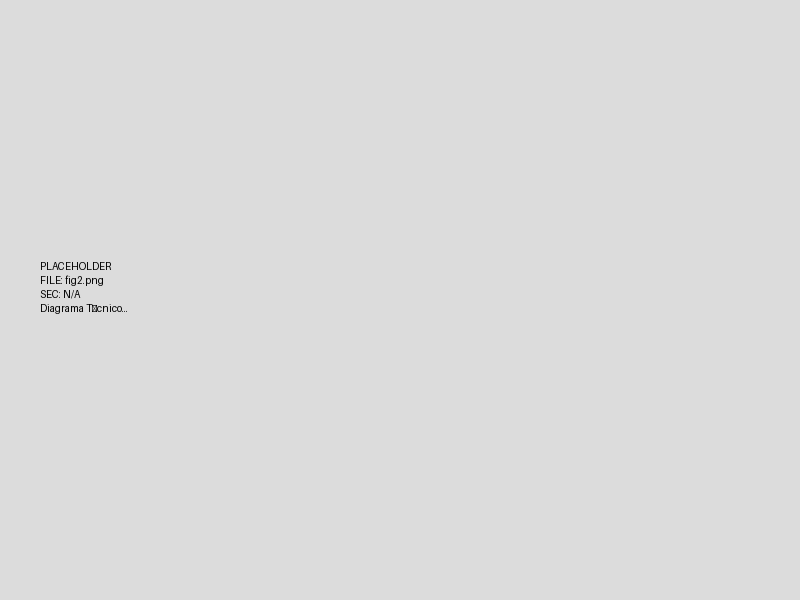
\includegraphics[width=\linewidth]{fig2.png}
\caption{Taxonomía de enfoques de criptografía post-cuántica, destacando familias basadas en lattices, códigos, multivariables y hash, con énfasis en suitability para entornos NB-IoT restringidos.}
\label{fig:taxonomia_pqc}
\end{figure}

En síntesis, el estado del arte muestra avances prometedores pero también brechas importantes. Mientras algunos algoritmos lattice-based demuestran viabilidad tras optimizaciones, persisten interrogantes sobre su integración fluida en stacks 3GPP existentes y su comportamiento en escenarios reales de exploración profunda. Estas limitaciones motivan directamente la propuesta que se desarrolla en las secciones siguientes.